\documentclass[sigconf,review]{acmart}

%%
%% \BibTeX command to typeset BibTeX logo in the docs
\AtBeginDocument{%
  \providecommand\BibTeX{{%
    \normalfont B\kern-0.5em{\scshape i\kern-0.25em b}\kern-0.8em\TeX}}}

\setcopyright{acmcopyright}
\copyrightyear{2019}
\acmYear{2019}
\acmDOI{10.1145/xxxxxxx.yyyyyyy}

\acmConference[SC19]
{The International Conference for High Performance Computing, Networking, Storage, and Analysis}
{November 17--22, 2019}{Denver, CO, USA}

\begin{document}

\title{What Deploying MFA Taught Us About Changing Infrastructure}

\author{Kelly L.\ Rowland}
\orcid{https://orcid.org/0000-0001-5147-0051}
\affiliation{National Energy Research Scientific Computing Center (NERSC)}
\email{kellyrowland@lbl.gov}

\author{Abe Singer}
\affiliation{National Energy Research Scientific Computing Center (NERSC)}
\email{abe@lbl.gov}

\author{Shane Canon}
\affiliation{National Energy Research Scientific Computing Center (NERSC)}
\email{scanon@lbl.gov}

\author{Rebecca Hartman-Baker}
\affiliation{National Energy Research Scientific Computing Center (NERSC)}
\email{rjhartmanbaker@lbl.gov}

\author{David Skinner}
\affiliation{National Energy Research Scientific Computing Center (NERSC)}
\email{deskinner@lbl.gov}

\author{Craig Lant}
\affiliation{National Energy Research Scientific Computing Center (NERSC)}
\email{clant@lbl.gov}

\begin{abstract}

abstract

\end{abstract}

\begin{CCSXML}
<ccs2012>
<concept>
<concept_id>10002978.10003029.10003032</concept_id>
<concept_desc>Security and privacy~Social aspects of security and privacy</concept_desc>
<concept_significance>500</concept_significance>
</concept>
<concept>
<concept_id>10002978.10003029.10011703</concept_id>
<concept_desc>Security and privacy~Usability in security and privacy</concept_desc>
<concept_significance>500</concept_significance>
</concept>
<concept>
<concept_id>10002944.10011122.10002947</concept_id>
<concept_desc>General and reference~General conference proceedings</concept_desc>
<concept_significance>100</concept_significance>
</concept>
</ccs2012>
\end{CCSXML}

\ccsdesc[500]{Security and privacy~Social aspects of security and privacy}
\ccsdesc[500]{Security and privacy~Usability in security and privacy}
\ccsdesc[100]{General and reference~General conference proceedings}

\keywords{multi-factor authentication, MFA, infrastructure}

\maketitle

\section{Introduction}

lorem ipsum MFA

\section{Goals}

lorem ipsum MFA

\section{Requirements}

lorem ipsum MFA \cite{xie2013fast, diffie1977special}

\section{Solutions}

lorem ipsum MFA

\begin{figure*}[h]
  \centering
  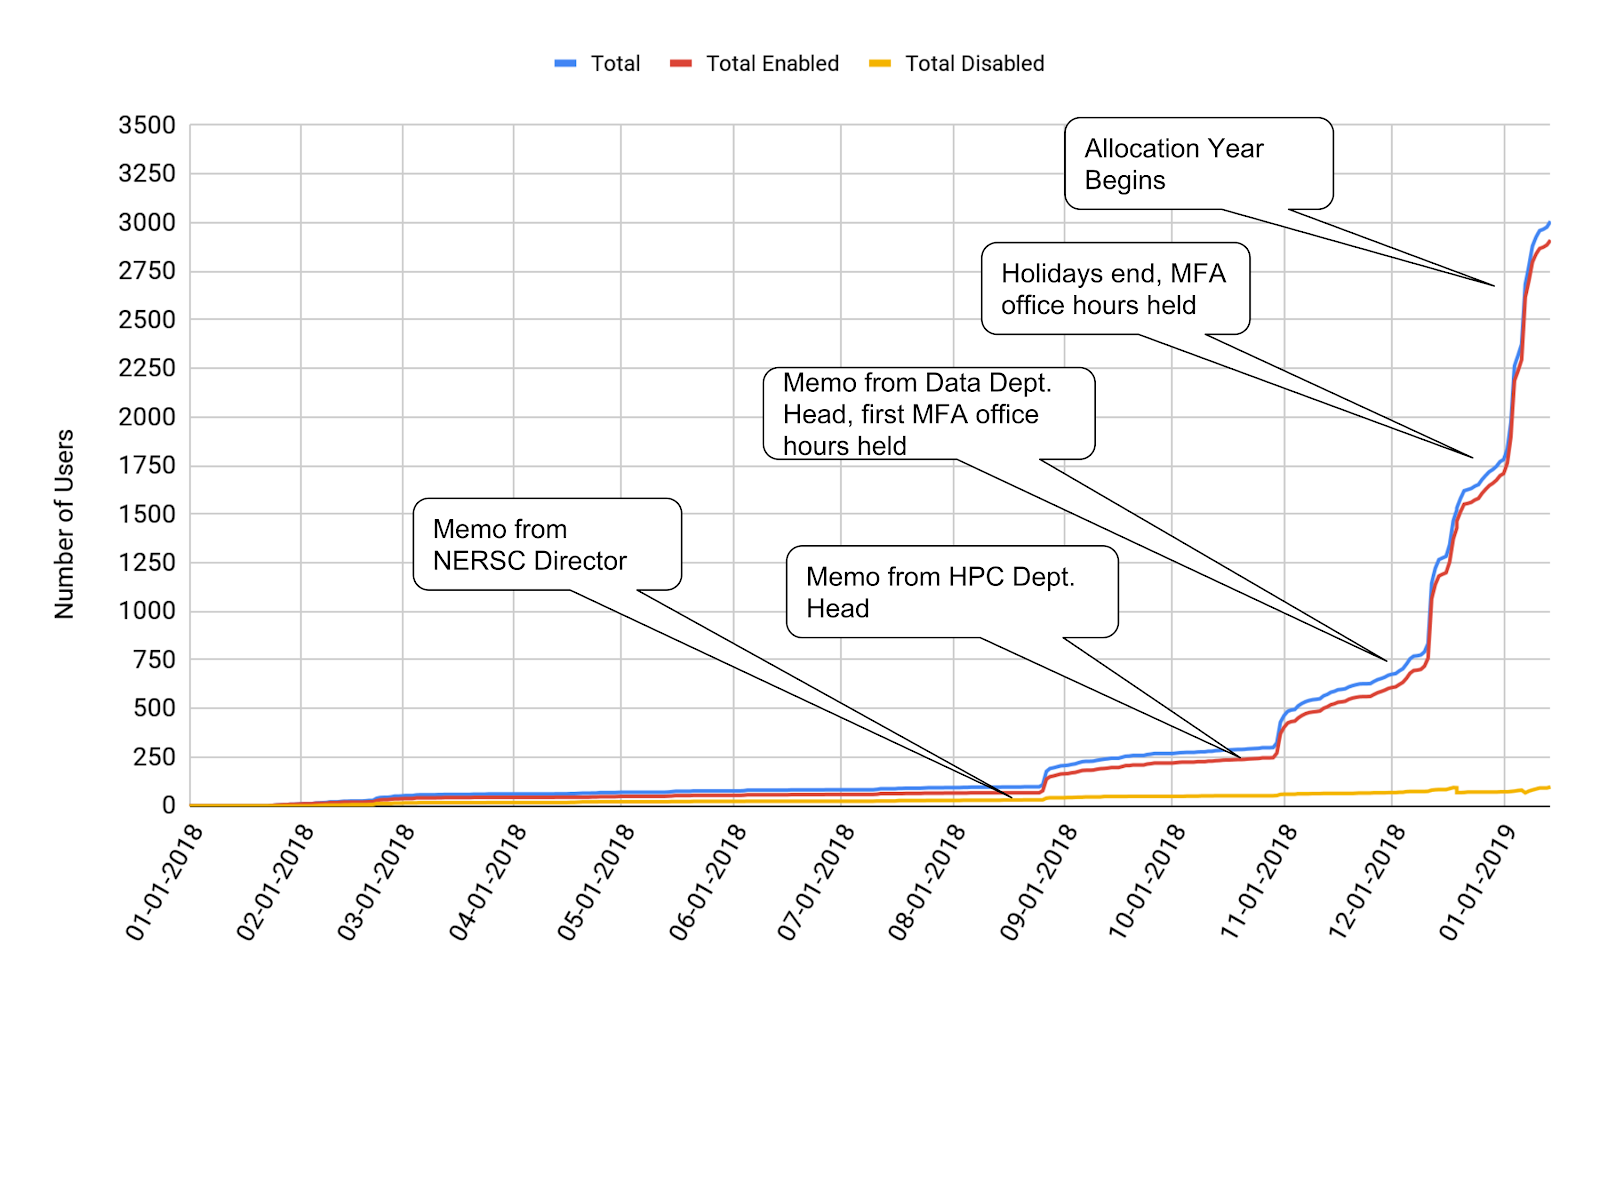
\includegraphics[width=\textwidth]{uptake.png}
  \caption{User enrollment in MFA in 2018, from initial rollout to mandatory requirement.}
  \Description{User enrollment in MFA in 2018, from initial rollout to mandatory requirement.}
\end{figure*}

\section{Conclusions and Future Work}

lorem ipsum MFA

%%
%% The next two lines define the bibliography style to be used, and
%% the bibliography file.
\bibliographystyle{ACM-Reference-Format}
\bibliography{hpcsyspros19}

\end{document}
